\section {Carboxylic Acid Orientation}

Calculations were performed to characterize the orientation and geometry of succinic acid with respect to its position relative to the water surface. Figure \ref{fig:angle-definitions} depicts the succinic acid molecule and shows two angle definitions relative to the surface normal (labeled ``z''). The angular tilt, $\theta$, is the angle between the O-C-O bisector axis of the carboxylic acid head group and the vector normal to the plane of the water surface. $\theta$ varies from being aligned with the surface normal, to 90$^{\circ}$ and in the plane of the surface, to 180$^{\circ}$ anti-aligned with the surface normal ($0^{\circ} \le \theta \le 180^{\circ}$). The carboxylic acid group twist, $\phi$, measures the angle between the plane of the O-C-O of the carboxylic acid, and the plane formed by the O-C-O bisector and the surface normal. This is the same as the dihedral defined by three vectors: The surface normal, the O-C-O bisector axis, and the vector from the carbon to the carbonyl oxygen of the acid group. $\phi$ can take values of $-180^{\circ} \le \phi \le 180^{\circ}$, where a value of $0^{\circ}$ aligns the carbonyl oxygen with the plane of the surface normal, and a value of 90$^{\circ}$ place both the carbonyl and alcohol oxygens in the plane of the water surface. A third angle, $\psi$, is the dihedral angle of the carbon backbone, where $\psi = 0^{\circ}$ puts the succinic acid into a ``trans-'' carbon-chain configuration. The full range of dihedral twists is folded into $0^{\circ} \le \psi \le 180^{\circ}$ because of the symmetry of the succinic acid. 

\begin{figure}[h!]
	\begin{center}
		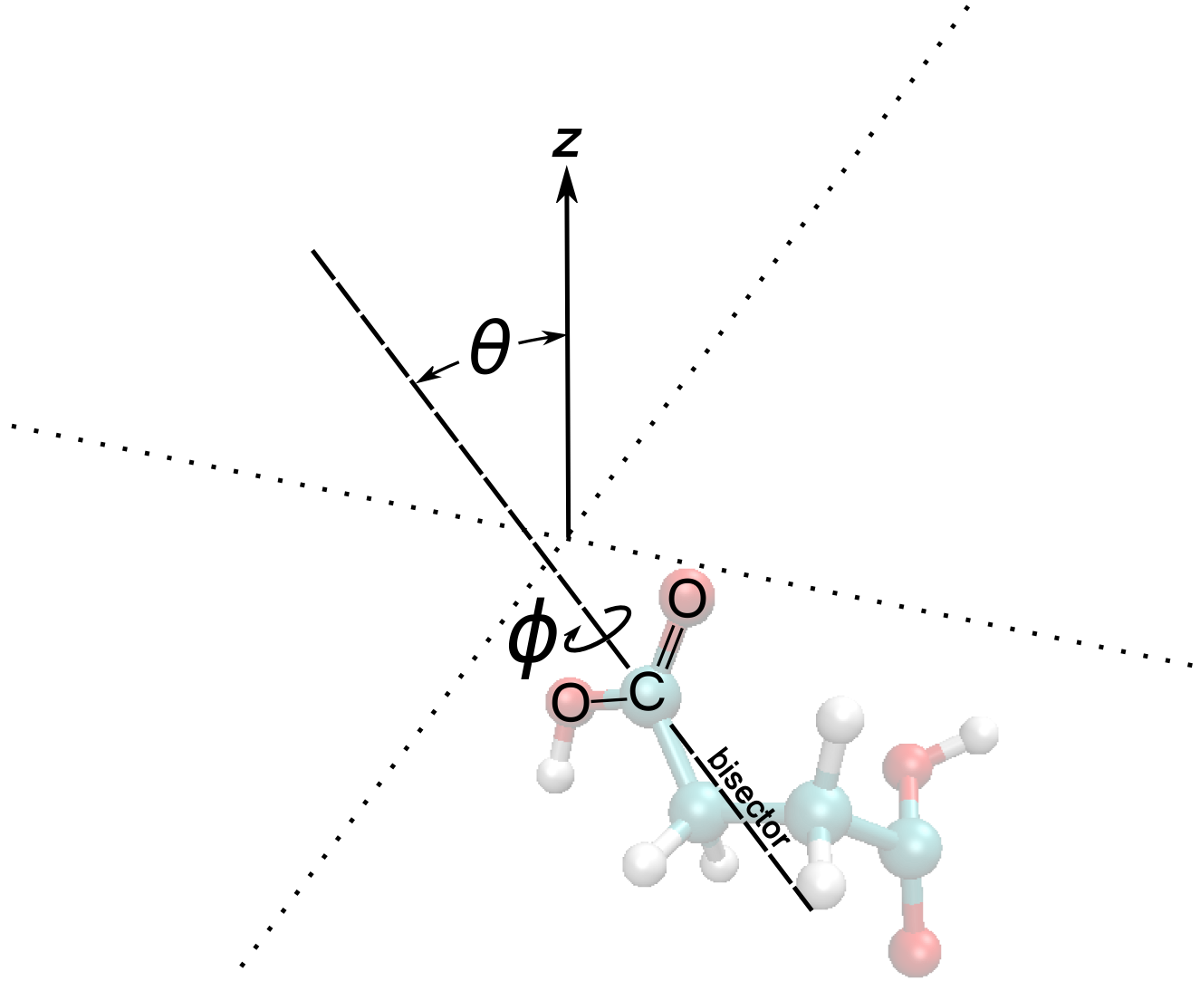
\includegraphics[scale=1.0]{images/bond-angles/bond-angle-definitions-small.png}
		\caption{}
		\label{fig:angle-definitions}
	\end{center}
\end{figure}

We first look at the dihedral angle to understand the twist of the carbon backbone at different locations in the interface. Figure \ref{fig:dihedral} is an angular depth profile of the dihedral angle, $\psi$, on the y-axis, plotted against the distance of the molecular center of mass to the water surface on the x-axis. Positions further into the water bulk appear on the left of the plot. The coloration ranges from dark blue to red, indicating low and high intensities of the 2D histogram, respectively. Clearly the molecule mostly has a $\psi$ value centered at $60^{\circ}$ at all depths, with minor contributions from the cis-configuration of the carbon backbone at $\psi = 180^{\circ}$. The greatest contribution is from the gauche configure of the acid groups. The $180^{\circ}$ configuration is represented throughout the deeper regions of the interface and in the water bulk. Near -2\angs~and further towards the surface, the distribution completely shifts to the $60^{\circ}$ gauche configuration. The succinic acid molecules within approximately 2\angs of the surface location have a strong preference for a gauche dihedral configuration. 

\begin{figure}[h!]
	\begin{center}
		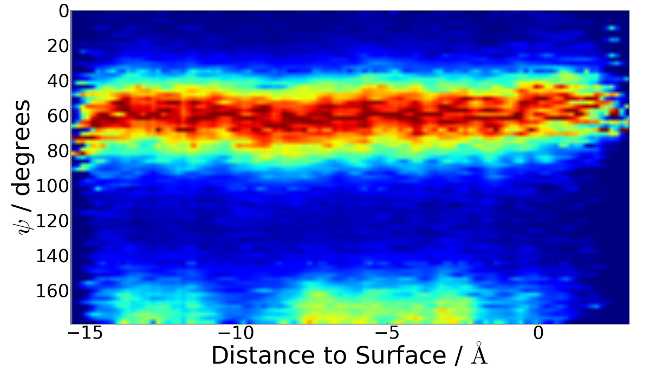
\includegraphics[scale=1.0]{images/dihedral/dihedral-small.png}
		\caption{}
		\label{fig:dihedral}
	\end{center}
\end{figure}

% Tilt/Twist
\begin{figure}[h!]
	\begin{center}
		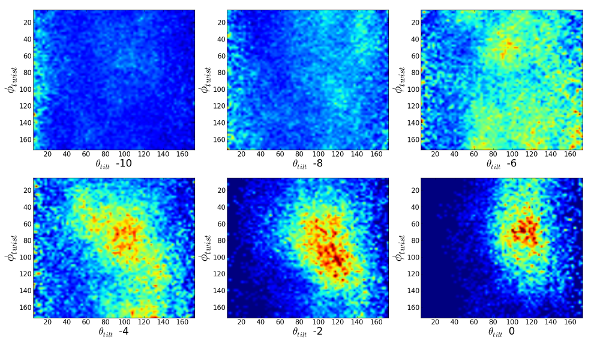
\includegraphics[scale=1.0]{images/bond-angles/carbonyl-tilt-twist-small.png}
		\caption{}
		\label{fig:tilt-twist}
	\end{center}
\end{figure}
